\documentclass[10pt]{article}
\usepackage[polish]{babel}
\usepackage[utf8]{inputenc}
\usepackage[T1]{fontenc}
\usepackage{amsmath}
\usepackage{amsfonts}
\usepackage{amssymb}
\usepackage[version=4]{mhchem}
\usepackage{stmaryrd}
\usepackage{graphicx}
\usepackage[export]{adjustbox}
\graphicspath{ {./images/} }

\newcommand\Varangle{\mathop{{<\!\!\!\!\!\text{\small)}}\:}\nolimits}

\begin{document}
\begin{enumerate}
  \item Czworokąt wypukły \(A B C D\) jest wpisany w okrąg.\\
Półproste \(A D\) i \(B C\) przecinają się w punkcie \(P\). Wykazać, że \(\Varangle A P B=|\Varangle A D B-\Varangle C A D|\).\\
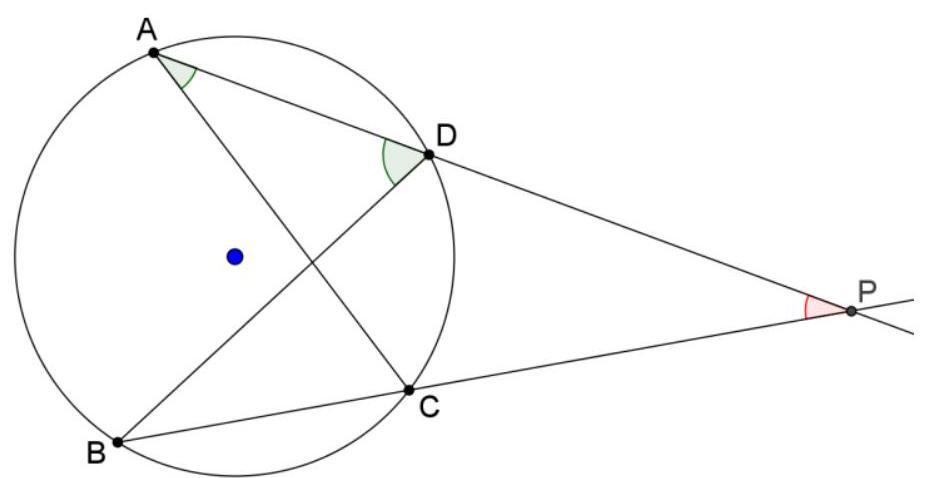
\includegraphics[max width=\textwidth, center]{2024_11_21_beb13eed4633d22d0b6ag-1}
  \item Punkty \(A, B\) i \(C\) leżą na jednej prostej (w podanej kolejności), przy czym \(A B<B C\). Punkty \(D\) i \(E\) są wierzchołkami kwadratu \(A B D E\). Okrąg o średnicy \(A C\) przecina prostą \(D E \mathrm{w}\) punktach \(P\) i \(Q\) ( \(P\) leży na odcinku \(D E)\). Niech \(R\) będzie punktem przecięcia prostych \(A Q\) i \(B D\). Wykazać, że \(D P=D R\).\\
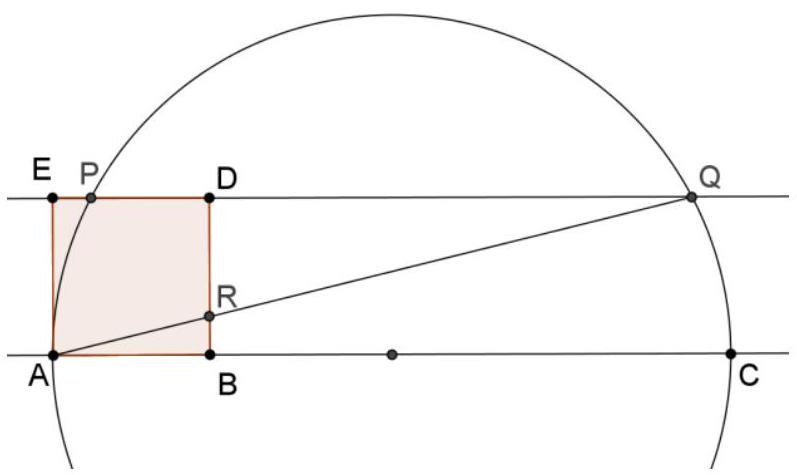
\includegraphics[max width=\textwidth, center]{2024_11_21_beb13eed4633d22d0b6ag-1(1)}
  \item Rozwiąż układ równań
\end{enumerate}

\[
\left\{\begin{array}{l}
x^{2}+9=4 y \\
y^{2}+1=6 z \\
z^{2}+4=2 x
\end{array}\right.
\]


\end{document}